%% Verze pro oboustranny tisk:
% Okraje: 
% (ale pozor, LaTeX si prida 1in)
\documentclass[10pt,a5paper]{article}
\usepackage[czech,english]{babel}
\usepackage[a5paper,margin=10mm]{geometry}
\newgeometry{top=20mm,bottom=20mm,right=15mm,left=15mm}
%\setlength\textwidth{102mm}
%\setlength\textheight{145mm}
%\setlength\oddsidemargin{0mm}
%\setlength\evensidemargin{0mm}
%\setlength\topmargin{0mm}
%\setlength\headheight{5mm}
%\setlength{\headheight}{15pt}
%\setlength{\parindent}{1cm}
\usepackage{pdfpages}
\usepackage{textcomp}

\usepackage[utf8]{inputenc}

\usepackage{bibentry}
\usepackage{url}
\usepackage[nottoc]{tocbibind}
\nobibliography*

\usepackage{titlesec}  %vzhled titulku prvni stranky kapitoly
%\let\footruleskip\undefined
\usepackage{fancyhdr}  %hlavicky stranek 

%% Ostatn� bal��ky
\usepackage{graphicx}
%\usepackage{amsthm} % for mathematical theorems, lemma, proof
\usepackage{amsmath} % for mathematical equation
\usepackage{amssymb} % for special symbols - blacktriangledown
%\usepackage{palatino} % font
%\usepackage{bookman} % another font
\usepackage[sc]{mathpazo} %palladio font
\usepackage[scaled]{helvet}
\usepackage{eulervm}

%\usepackage{setspace} % for linespacing
%\linespread{1.0}%\sin­glespac­ing %\onehalfspacing 
\usepackage[T1]{fontenc} %font encoding e.g. for czech characters
%\usepackage{diagbox} %diagonala v tabulce
%\usepackage{multirow} %viceradkove tabulky
%\usepackage[font=footnotesize]{caption} %velikost fontu v popisu
%\usepackage{etoolbox} %pro pozdejsi definici zpetne reference
%\usepackage[titletoc]{appendix} %appendices with names
%\usepackage{listings,multicol} % for code listings, multicolumned
%\lstset{% escape sequence inside listing
%  escapeinside={(*}{*)},%
%}
%\usepackage{dtsyntax} % for listings modelica
%\usepackage[version=3]{mhchem} % for writing chemical compounds and reaction
%\usepackage{siunitx} % formating numbers
%\renewcommand{\ttdefault}{pcr} % nicer font - courier in listing
\usepackage[unicode,colorlinks,backref=page]{hyperref}   % Musi byt za vsemi ostatnimi balicky
\hypersetup{pdftitle={Utilization of GRID in processing of medical information},
            pdfauthor={Tomáš Kulhánek},
            plainpages=false,
            urlcolor=blue,
            linkcolor=blue,
            citecolor=blue
            }

%\overfullrule=2cm %vyznacit na okraji, kde se nepodarilo zarovnat
%definice jak ma vypadat zpetna reference
%\makeatletter
%\patchcmd{\BR@backref}{\newblock}{\newblock(cited on p.~}{}{}
%\patchcmd{\BR@backref}{\par}{)\par}{}{}
%\renewcommand\bibentry[1]{\nocite{#1}{\frenchspacing
%     \@nameuse{BR@r@#1\@extra@b@citeb}}}
%\makeatother
\makeatletter
\def\@makechapterhead#1{
  {\parindent \z@ \raggedright \normalfont
   \Huge\bfseries \thechapter. #1
   \par\nobreak
   \vskip 10\p@
}}
\def\@makeschapterhead#1{
  {\parindent \z@ \raggedright \normalfont
   \Huge\bfseries #1
   \par\nobreak
   \vskip 10\p@
}}
\makeatother

\begin{document}
\shorthandoff{-} % fix problems with babel czech and includepdf chars '-' 
\pagenumbering{arabic} %first pages with roman numbering
\setcounter{page}{1}
%\lefthyphenmin=2
%\righthyphenmin=2
\pagestyle{empty} % title page without number
%\singlespacing 
%\sin­glespac­ing % 1.0 row space
\begin{center}
%\singlespacing 
\large
%\begin{tabular}{rl}
\textbf{\Large{Univerzita Karlova v Praze}}

\textbf{\Large{1.lékařská fakulta}} 

\textit{Charles University in Prague} 

\textit{1st Faculty of Medicine}
%\end{tabular}
\vfill
\normalsize
\begin{tabular}{rl}
Studijní obor:  & Biomedicínská informatika \\
\noalign{\vspace{-1mm}}
\textit{Study domain} & \textit{Biomedical informatics} \\
\end{tabular}

\vfill

{\Large Autoreferát dizertační práce}

\textit{\large Summary of the dissertation}


\centerline{\mbox{\includegraphics[width=50mm]{../img/logouk.png}
\includegraphics[width=50mm]{../img/logolf1.png}}}


\vfill



% N�zev pr�ce p�esn� podle zad�n�
\textbf{\large Využití technologie GRID při zpracování medicínské informace}

\vspace{2mm}
\textit{\large Utilization of GRID technology in processing of medical information}
\vfill
{\Large Mgr. Tomáš Kulhánek}

% N�zev katedry nebo �stavu, kde byla pr�ce ofici�ln� zad�na
% (dle Organiza�n� struktury MFF UK)
% CESNET z.s.p.o., Institute of pathological physiology



\vfill

Praha 2015

\end{center}


%\frontmatter
%\onehalfspacing %1.5 row space
\newpage
\selectlanguage{czech}
%\normalsize
\begin{center}
\textbf{Doktorské studijní programy v biomedicíně}

\textit{Univerzita Karlova v Praze a Akademie věd České republiky}
\end{center}
\normalsize

\vspace{2mm}

Obor: Biomedicínská informatika
\vfill
Předseda oborové rady: Prof. RNDr. Jana Zvárová, DrSc.
\vfill

Školicí pracoviště: CESNET z.s.p.o., Ústav patologické fyziologie 1.LFUK
\vfill


Školitel:  Ing. Milan Šárek, CSc.
\vfill

Konzultant:  Doc. MUDr. Jiří Kofránek, CSc. 
\vspace{100mm}

Disertační práce bude nejméně pět pracovních dnů před konáním obhajoby zveřejněna
k nahlížení veřejnosti v tištěné podobě na Oddělení pro vědeckou činnost a zahraniční styky
Děkanátu 1. lékařské fakulty.


%
\newpage
\selectlanguage{english}

\begin{center}
\Large \textbf{Dedication}
\end{center} 
\vfill
\begin{center}
To my beloved children Karla and Matěj and my dearest lovely wife Marie,

without whom this work would not have been completed.
\end{center} 
\vfill
\newpage
\mbox{}
\newpage
\pagestyle{plain} % other pages with number
\begin{center}
\Large \textbf{Acknowledgements}
\end{center} 
I would like to express my gratefulness to my supervisor Ing. Milan Šárek, CSc. for his support and guidance throughout the beginning of my research. 
I would also like to thank the staff of association CESNET, especially Ing. Jiří Navrátil, CSc., who gave me an opportunity to work with computing resources connected via high speed academic network and to follow the development of the networking technologies. Further thanks go to the staff of METACENTRUM, department of CESNET, for giving support and access to powerful computing infrastructure for scientific purposes. I would like to thank to the staff of EGI.eu, who gave me an opportunity to be EGI Champion, selected users of scientific European grid-computing and cloud-computing infrastructure. This made me possible to meet the most inspiring people in the technology domain as well as scientific domain face to face. 

I would like to thank the fellows from Musical Acoustic Research Center of Academy of Performing Arts, especially RNDr. Marek Frič, PhD. and Ing. Zdeněk Otčenášek, Phd. for their inspiring atmosphere in the research domain of voice science. 

I would like to thank my colleagues from Laboratory of Biocybernetics and Computer Aided Teaching within Institute of Pathological Physiology including Mgr. Marek Mateják, Ing. Jan Šilar, Ing. Filip Ježek, Ing. Martin Tribula and MUDr. et Mgr. Pavol Privitzer, who provided me pleasure and inspiring atmosphere for my research and development work during the second part of my research. Especially, I would like to thank to my consultant Doc. MUDr. Jiří Kofránek, CSc. and a fellow MUDr. Stanislav Matoušek, PhD., who taught me the subject of medical physiology and who guided me within the topic of mathematical models and simulation of integrative physiology. Last but not least, thanks to Veronika Sýkorová, DiS and Klára Ulčová, DiS for their help with graphical schemas. 

The research projects were solved within the cooperation between association CESNET, First Faculty of Medicine of Charles University in Prague and Academy of Performing Arts in Prague and was partially supported by the project of Ministry of Education, Youth and Sport of the Czech Republic MSM6383917201, by the projects of Development Fund of CESNET 2009/361, 2010/384, 2011/423, 2011/431 and by the project of Ministry of Industry and Trade of the Czech Republic MPO FR-TI3/869.

\newpage
\mbox{}

%\pagestyle{plain} % other pages with number
%\mainmatter

\tableofcontents

\newpage
\section*{Abstrakt}
\addcontentsline{toc}{section}{Abstrakt (česky)}


%%% Povinn� informa�n� strana diserta�n� pr�ce

\vbox to 0.5\vsize{
\setlength\parindent{0mm}
\setlength\parskip{5mm}
\selectlanguage{czech}
\textbf{Název práce:}
Využití technologie GRID při zpracování medicínské informace

\textbf{Autor:}
Mgr. Tomáš Kulhánek

\textbf{Katedra,ústav: }
Ústav patologické fyziologie 1.LFUK  

\textbf{Školitel:}
Ing. Milan Šárek, CSc., CESNET z.s.p.o.

\textbf{Konzultant:}
Doc. MUDr. Jiří Kofránek, CSc.

\textbf{Abstrakt:}

Práce prezentuje výzkum a výsledky využití technologií, které umožňují sdílet výpočetní a úložné kapacity a to v oblasti biomedicínského výzkumu. Vedle technologie GRID se rozvíjí virtualizačních technologie (VMWare, XEN, ...), které dodali distribuovaným systémům novou vlastnost zdání vlastnictví a přímé kontroly konfigurovatelné infrastruktury jako služby, jež se dnes shrnují pod společný pojem CLOUD computing. V práci jsou diskutovány teoretické limity distribuovaných systémů a paralelních výpočtů v nich tak i praktické výsledky ve vybraných oblastech. V oblasti výměny medicínských snímků a souvisejících zdravotních záznamů byla ukázána snadná integrovatelnost se stávajícími systémy při respektování požadavků na bezpečnost dat. V oblasti analýzy a zpracování lidského hlasu v reálném čase byla ukázána možnost poskytování nadstandardních výpočetních služeb pro komunitu uživatelů. V oblasti modelování fyziologických systémů je prezentován systém pro odhad parametrů a identifikaci fyziologických systémů komplexních modelů, které by byli obtížně řešitelné za použití klasických metod.

\textbf{Klíčová slova:}

grid-computing, cloud-computing, matematické modelování, výpočetní fyziologie, fonetogram
% 3 a� 5 kl��ov�ch slov

\vss}

\newpage
\section*{Abstract}
\addcontentsline{toc}{section}{Abstract}
\newpage

\nobreak\vbox to 0.49\vsize{
\setlength\parindent{0mm}
\setlength\parskip{5mm}
\selectlanguage{english}
\textbf{Title:}
Utilization of GRID technology in processing medical information

\textbf{Author:}
Tomáš Kulhánek

\textbf{Department:}
Institute of pathological Physiology

\textbf{Supervisor:}
Ing. Milan Šárek, CSc., CESNET z.s.p.o

\textbf{Consultant:}
Doc. MUDr. Jiří Kofránek, CSc.

\textbf{Abstract:}

Two work presents results, which are researched in the field of utilization technology who offers distributed computing and storage capacity to exchange medical information, demanding computation and data exchange. Next to the GRID technology. The virtualization technology evolved and were utilized more massively next to the GRID technology and these gives distributed systems a new quality and services called today with the name CLOUD. This work summarizes result of different projects which implements selected technologies in the field of GRID and CLOUD to systems which are used in medical education and research and in neighboring fields. The multidisciplinary projects were solved within the cooperation between association CESNET, First Faculty of Medicine of Charles University in Prague and Academy of Performing Arts in Prague.

% abstrakt v rozsahu 80-200 slov v angli�tin�; nejedn� se v�ak o p�eklad
% zad�n� diserta�n� pr�ce

\textbf{Keywords:}
grid, cloud, computational physiology, phonetogram
% 3 a� 5 kl��ov�ch slov v angli�tin�

\vss}


%\small
%\pagenumbering{arabic} %thesis pages with arabic numering
%\setcounter{page}{1}

\pagestyle{fancyplain}
\fancyhf{}
%\lhead{ \fancyplain{}{\leftmark} }
\fancyhead[LE]{ \fancyplain{}{\leftmark} }
%\fancyhead[RE]{ \thepage }
\fancyhead[RO]{ \fancyplain{}{\leftmark} }
%\fancyhead[LO]{ \thepage }

\cfoot{ \thepage }


\chapter{Introduction}

\emph{Grid computing} is usually defined as sharing computational and data storage resources across organizational boundaries which can give a user much more computational or storage capacity. Grid computing in contrast to common distributed computing focus on large-scale resource sharing. The technology under grid computing provides access to a computational resources in a federated way, while preserving some rights of the owner. Requirements, standards and architecture, were proposed and published, e.g., by Foster et al. \cite{Foster2001, Foster2003} and such infrastructures are currently distinguished as "service" grids. It's non-trivial task to maintain scientific grid, thus specialists from the so-called national grid initiatives (NGI)\nomenclature{NGI}{National Grid Initiative} maintains and cooperates with similar grid initatives of other countries. In Europe these are coordinated, e.g., by European Grid Infrastructure (EGI)\nomenclature{EGI}{European Grid Infrastructure}. One of the largest project computed in these grid infrastructures are related to experiments of high-energy physics in order to process a large number of observed data in a reasonable time \cite{Bird2009}. The Worldwide Large Hadron Collider Computing Grid (WLCG)\nomenclature{WLCG}{Worldwide Large Hadron Collider Computing Grid} was designed to store and process almost 30 PetaBytes of data per year in the period of 2009-2013  \cite{Adamova2014}.

Another approach to grid computing is joining desktop computers from an individual user to form a voluntary or desktop grid. It was popularized by a project that tries to identify uncommon signals from space to search for extraterrestrial intelligence (SETI@Home)\footnote{\url{http://setiathome.ssl.berkeley.edu/}}\cite{Anderson2002}. And general-purpose frameworks were built in order to facilitate the development of projects that use a similar philosophy of computing on desktop computers, e.g., BOINC\nomenclature{BOINC}{Berkeley Open Infrastructure for Network Computing} \cite{Anderson2004} and others.

In recent years, the development of virtualization technologies has enhanced the availability of services that are provided by grid computing. It has additionally enabled an evolution of the so-called \emph{cloud computing}, in which computing resources can be rapidly provisioned and released with minimal management effort or service provider interaction. This implicates important feature of cloud-computing -- elasticity -- ability to scale up and down computing resources when required \cite{Mell2011}. The cloud computing is provided in several models, however, currently the scientific infrastructures offer mainly Infrastructure as a Service (IaaS)\nomenclature{IaaS}{Infrastructure as a Service}, which offers the whole virtual infrastructure including virtual machine and network accessible for user per request.

With respect to technology development available in scientific infrastructures, this thesis focus not only on grid computing but also on cloud computing technology, which were available for scientific computing within grid infrastructures since 2012.
 %This work focuses on processing of medical information should give enhanced information, which can be analysed easily. Thus further analysis or synthesis of such information is beyond this work, so the aim is not to give particular results on some specific diseasies, pathologies etc., however, with cooperation of other experts it is a desired side effect.

%The author's work was published in a series of peer-reviewed papers of international journals and peer-reviewed conference proceedings \cite{kulhanek2009, kulhanek2010b, kulhanek2010c,  Kulhanek2014Parameters, Kulhanek2014Modeling, Kulhanek2014mefanet, Matejak2014sj} which are included in this work as appendices. The author's work and contribution was also presented in international conferences and published in the respective proceedings and transactions \cite{Kulhanek2010, Kulhanek2013c, kofranek2013hummod, Matejak2014}. The work was also popularized in local and regional conferences and their respective proceedings \cite{Kulhanek2008Mefanet, Sarek2009, kulhanek2009dd, Kulhanek2009Mefanet, Kulhanek2010d, Kulhanek2010Mefanet, Kulhanek2011, kulhanek2011dd, Kulhanek2012, Kulhanek2013b, Kulhanek2014, Kulhanek2012a}. The author contributed to the utility model, which was registered by the Czech Industrial Property Office \cite{Kofranek2014a}.

 %intro
\section{Hypothesis}
To summarize this section. If there will be technological speedup, this will impact mainly the class of problems which are solvable by polynomial algorithm. For the problems where the computation needs tremendous ammount of time, because current known algorithm is exponential, there can be used non-exact methods to find at least some solution if not the exact one. 
\begin{itemize}
\item{The \emph{heuristic methods} tries to eliminate the number of steps of computation by some implicit or explicit knowledge of the specific problem itself E.g. eliminating solution classes that seems not to go to optimal solution. With combination of brute-search the heuristic methods reduce the size of all possible solution candidates to check.}
\item{The \emph{randomization methods} use non-deterministic methods in some level of computation.E.g. Monte-Carlo method is used to compute problems using pseudo-random generated values and after several iterations statistical methods are used to compute expected value and standard deviation. }
\item{\emph{Restriction on input data} - is another form of using the explicit knowledge of the problem instance ad it may reduce all possible values to be checked. }
\item{\emph{Approximation algorithm} - may find not only some good solution, but can quantify how far from the optimal solution the found is good with some degree of probability.}
\end{itemize}

To summarize this section; parallel computing can introduce speedup on current computational technology and some computation problems may become feasible.
Also overhead caused by parallelization and fraction of non-parallelizible parts should be considered as it may degrade expected speedup.
In case of exponential algorithm (e.g. for NP-complete problems) the speedup will increase the size of solvable problem only slightly (see table \ref{table:speedupeffect}) and some problems cannot be (or it is believed) significantly speedup by parallel computing. 
In further text a focus will be given mainly to task parallelism and distributed computing. 

\section{Distributed computing technologies}
\label{sec:distributed}

Distributed computing is based on the idea to spread the computation task into set of computers which are connected via computational network.
 %hypothesis
\chapter{Methods}

From a computer science (informatics) point of view, it is assumed that the processing of medical information is, in general, a computational problem, which is understood as a task that can be solved by a computer. An algorithm is a set of operations that is used to accomplish tasks and solve problems. 
The important features of an algorithm are effectivity (what is the time complexity of the algorithm regarding the size of input data) and scalability (how far can an algorithm benefit from parallel computing). Grid computing and cloud computing brings a technology that enables parallel computing in a large amount of shared computers, servers or cluster of servers introduces large speedup of computation and can decrease the time of computation substantially. However, problems solvable by algorithms with exponential time complexity (e.g. NP-hard or NP-complete\nomenclature{NP-complete}{Nondeterministig Polynomial - complete}) can't be addressed by any large scale infrastructure \cite{Garey1979}. Therefore, additional non-exact methods for such type of problems are used to obtain at least some solution including heuristic method (eliminate some steps or solution classes that seems to not go to optimal solution), randomization (pseudo random values are generated and statistical methods can be used to compute expected optimal value) and others. 

\section{Sharing Medical Images}
The DICOM standard\footnote{DICOM: \url{http://dicom.nema.org/} accessed January 2015}\nomenclature{DICOM}{Digital Imaging and Communication Protocol} was used as a joint protocol to integrate grid-based system Globus MEDICUS \cite{Erberich2006} with current production system MEDIMED for sharing medical images among different hospitals \cite{Slavicek2010}, which is based on common distributed system with central cluster. 
% which may suffer with single point of failure and bottleneck issues. 
Globus MEDICUS \cite{Erberich2006,Erberich2007} implements a DICOM Grid Interface Service (DGIS) and integrates the open-source PixelMed\texttrademark ~Java DICOM Toolkit\footnote{\url{http://www.pixelmed.com/} accessed February 2015} into a web service, communicating via the DICOM protocol. Furthermore, it forwards queries to the underlying services within Globus toolkit. The console application of the MEDIMED project can be interconnected via DICOM protocol with local Picture Archiving and Communication System (PACS)\nomenclature{PACS}{Picture Archiving and Communication System} and selected DICOM studies can be sent/retrieved to another institution connected to the MEDIMED project.




%The typical workflow of a medical image in a hospital is in Figure \ref{fig:pacs}. 
%\begin{figure}[ht]
%    \centering
%    \includegraphics[width=0.7\textwidth, height=8cm]{img/chapter3-pacs.png}
%    \caption{Data acquisition is made by modalities (magnetic resonance, ultrasonography, etc.). By using the DICOM format and protocol, it can be directly transferred and visualized by diagnostic workstation. With the metadata filled by an expert physician, the image is stored in PACS. Other desktops within the hospital can retrieve the image and review the report.}
%    \label{fig:pacs}
%\end{figure}
%When there is need to share medical data records including medical images among different institutions and hospitals, a challenge should be solved with data confidentiality and size of the data. The DICOM\footnote{DICOM: \url{http://dicom.nema.org/} accessed January 2015}\nomenclature{DICOM}{Digital Imaging and Communication Protocol} standard is used for exchanging medical images electronically.  Picture Archiving and Communication System (PACS)\nomenclature{PACS}{Picture Archiving and Communication System} holds the acquired DICOM images with metadata and description, which are  noted by experts. PACS is usually part of the information systems in hospitals.
%
%

%\section{Sharing Medical Images}
%Various tools are already available within current grid infrastructures, including open-source and licensed software for computation. The local scientific grid provider may give a list of the available applications\footnote{applications available in CESNET METACENTRUM \url{https://wiki.metacentrum.cz/wiki/Kategorie:Applications} accessed February 2015}. Alternatively, application databases are available in a broader environment, e.g., in the EGI.eu application database\footnote{\url{https://appdb.egi.eu/} accessed February 2015}.
%Additionally, the workflow systems and scientific gateways that are mentioned in section \ref{sec:introworkflow} try to hide the complexity of grid or cloud computing infrastructures and may also be used to integrate specific domains.
%In designing a new application, the programming model of parallel computing and/or distributed  computing (in section \ref{sec:parallelprogramming} and  \ref{sec:distributedprogramming}) needs to be followed, utilizing the benefits of grid computing and cloud computing.

%The general approach to port applications to a grid infrastructure is to automatize what can be automatized, i.e., make scripts, configure system, prepare some user interface, integrate with existing applications, utilize protocol compatibility, etc. Additionally, the prepared template, script or application should be reused for further similar computational requests.

%\section{Sharing Medical Images}
%\label{sec:imaging}
%
%Use cases that relate to digital medical images involve image acquisition, preprocessing, storing and searching \cite{Bankman2000}.
%
%The acquisition of a medical image is performed with different modalities (different types of equipment and sensors) by radiologists or other specialists. The DICOM\footnote{DICOM: \url{http://dicom.nema.org/} accessed January 2015}\nomenclature{DICOM}{Digital Imaging and Communication Protocol} format and protocol has become an industrial standard for exchanging medical images electronically and in Picture Archiving Communication Systems (PACS). PACS holds the acquired DICOM images with metadata and description, which are  noted by experts. PACS is usually part of the information systems in hospitals. Figure \ref{fig:pacs} shows the typical workflows of a medical image in a hospital.
%
%
%
%%To summarize this section, in past years, 
%Digital medical image acquisition, storing, exchanging and processing has become common and it currently uses distributed computing techniques\cite{Slavicek2010, Ross2010, Saliba2012}. Several efforts have been made to implement medical data management within grid or cloud infrastructures for research purposes\cite{Erberich2006, Duque, Montagnat2007, Krefting2009, Krefting2010}  and to integrate them with production infrastructures \cite{Skaburskas2008, Benkner2010} or to share knowledge in semi-formally described semantics \cite{Kuba2006}.
%
%The Globus toolkit belongs to a group of the most used grid middleware (see section~\ref{sec:servicegrid}). 
%%The core service included in Globus Toolkit is GridFTP -- grid extension to file transfer protocol(FTP)\nomenclature{FTP}{File Transfer Protocol}. This implements strategies such as \emph{stripping data} into multiple pieces; the \emph{parallel transfer of data}, utilizing stripped data parts to be transferred via different channels; \emph{partial file transfer}, some applications may not need to access the whole file but rather a smaller portion of it, etc., as described by Foster et al. and Allcock et al. \cite{Foster2006, Allcock2005}. Other core services are Replica Location Service, which aims to localize data, and Globus Resource Allocation Management (GRAM), which provides web service and proxies to the lower level job scheduler's implementation \cite{Foster2006}.
%%Next to core services, the domain-specific services might be implemented for the purpose of an application that uses the Open Grid Service Architecture (OGSA). 
%Globus MEDICUS \cite{Erberich2006,Erberich2007} implements a DICOM Grid Interface Service (DGIS) and integrates the open-source PixelMed\texttrademark ~Java DICOM Toolkit\footnote{\url{http://www.pixelmed.com/} accessed February 2015} into a web service, communicating via the DICOM protocol. Furthermore, it forwards queries to the underlying services within Globus toolkit. 
%
%%DGIS acts as a gateway to a grid infrastructure. As communication via the DICOM protocol is not secured, it is recommended that the DGIS be installed on the location of the PACS system or the DICOM ready modality or software. When a DICOM study is uploaded into DGIS, it is anonymized and stored. A record is made into another service’s Meta Catalog service, which resides in the same domain or anywhere in the grid that is accessible via the Globus Toolkit. Such an anonymized database of DICOM records can be used to query via the DGIS interface and to, for example, integrate with web-based applications, showing records for research purposes. Furthermore, authentication and authorization can be achieved in this level. 
%To integrate this system with an existing system MEDIMED project \cite{Slavicek2010} for sharing the medical images, the special client software "RediMed console", needs to be installed next to the DGIS. DGIS behaves as an access point to a PACS system whose records can be exchanged via the RediMed console software to other MEDIMED participants. 
%The results of this particular deployment and integration are presented in section \ref{sec:resultsimages}.
%
\section{Voice Science}
\label{sec:voice}

The software for parameterized Voice Range Profile (ParVRP) and Voice Range Profile in Real time (RealVoiceLab) was already developed and calibrated for selected types of microphones in an MS Windows platform by Fric et al. \cite{Fric2007,Fric2012}. Its implementation is carried out in an MATLAB environment, utilizing Signal Processing Toolbox\footnote{\url{http://www.mathworks.com/products/signal/} accessed February 2015}. It is compiled with a MATLAB Compiler and distributed as an executable. To migrate this legacy application into distributed environment, the virtualization can be used with a protocol to control an application remotely. Remote Desktop Protocol (RDP)\nomenclature{RDP}{Remote Desktop Protocol} is a proprietary protocol that is used for desktop sharing. It was primarily developed in a Microsoft Windows platform, however, today, clients and servers exist for several other platforms. RDP itself contains the redirection of several services, e.g., audio, sound recording, drive access, etc. 

%With the introduction of objective data analysis and laryngoscopy methods, voice science emphasized the cooperation among laryngologists, speech pathologists and voice teachers.
%The normal human voice ranges from 50 Hz to about 1~000 Hz and there are some  individual variations. For the analysis of a digitally recorded voice, either habitual or singing, the Discrete Fourier Transformation (DFT)\nomenclature{DFT}{Discrete Fourier Transformation} is used to produce a frequency and amplitude analysis of the recorded input voice samples. One of the most used class algorithm to compute DFT is the class of Fast Fourier Transformation (FFT)\nomenclature{FFT}{Fast Fourier Transformation} with computational complexity $O(n \log(n))$ \cite{Cooley1965,Frigo2005}.
%% and parallel version of the algorithms may introduce additional speedup for larger samples of analyzed data \cite{Gupta1993,Takahashi2003}. 
%The result of the analysis can be visualized in a voice range profile (VRP)\nomenclature{VRP}{Voice Range Profile} (Figure \ref{fig:vrp} and the significant difference between an untrained and trained voice can be seen, as published, e.g., by LeBorgne and Weinrich showing a signficant difference of VRP after nine-month training \cite{DeLeoLeBorgne2002}. Furthermore, some disorders can be quantitatively seen, which were published, e.g., by Wuyts et al.\cite{wuyts2003effects}.
%\begin{figure}[ht]
%    \centering
%    \includegraphics[width=0.8\textwidth, height=8cm]{img/autoreferat-vrp.png}
%    \caption{Voice Range Profile shows maximum and minimum intensity levels (y-axis) across the vocal range (x-axis) of normal speech (area surrounded by blue line) and singing (area surrounded by brown line).
%    }
%    \label{fig:vrp}
%\end{figure}
%
%%Another method that is used to analyze vocal chords is laryngoscopy. The videostroboscopy and high speed video in laryngoscope methods produce videos showing real movement of vocal chords. The videokymography method, introduced by Švec et al., complements the videostroboscopy. It allows the visualizing and analyzes of the movement of vocal cords. These movements are recorded by a high speed camera and an new image constructed from selected line of recorded video, which can be shown on standard TV or monitor using low frequency \cite{Svec1996,Svec2007}. 
%
%%In the case of a recorded sound and further analysis, there is a question about how such a service can be integrated in a grid computing or cloud computing environment in order to provide access to a complex application for non-technical voice specialists. Additionally, analytical software was already developed and calibrated for selected types of microphones in the MS Windows platform by Frič et al. \cite{Fric2007,Fric2012}. Therefore, I proposed and implemented a method that provides remote access to the analytical software. Section \ref{sec:methodsvoice} describes how the analytical software was customized with a remote desktop protocol (RDP)\nomenclature{RDP}{Remote Desktop Protocol}. Results are described in section \ref{sec:resultsvoice}. A similar approach can be used for processing  video recordings from a laryngoscope, however, the practical limits are discussed in section \ref{sec:conclusion}. 
%
%%\subsection{Methods for Remote Analysis of the Human Voice}
%\label{sec:methodsvoice}
%Terminal access to some remote computational capabilities, e.g., remote command-line or remote execution, is another integration strategy that is used for some remote infrastructures. Secure Shell (SSH) is used to establish a secure channel via an unsecured network (e.g., the Internet) from an SSH client to a SSH server. This is a basic method that is used to access a grid computing infrastructure. 
%Remote Desktop Protocol (RDP)\nomenclature{RDP}{Remote Desktop Protocol} is a proprietary protocol that is used for desktop sharing. It was primarily developed in a Microsoft Windows platform, however, today, clients and servers exist for several other platforms. Next to remote command-line, remote execution allows the accessing of remote graphical desktop environments. 

%
%%The computation of frequencies and amplitude from the recorded samples utilizes the effective Fast Fourier Transformation, which has time complexity $O(n\log(n))$. The benefit of deploying such an application in distributed infrastructures is the immediate access to updated software. Additionally, a collection of anonymized records of voice samples and results are very useful for further research and education. The possible disadvantage is the need to access to Internet.
%
%%This type of application can be packaged as a virtual machine template and configured within different types of cloud infrastructures. Together with a script or web portal, the on-demand deployment can be automated. The client part (RDP client) needs to connect to the appropriate instance. The results of such a deployment are discussed in section~\ref{sec:resultsvoice}.
%
\section{Computational physiology}
\label{sec:models}
A mathematical formalization of the fundamental knowledge and relation among a biological system – a mathematical model - is used as a base abstraction in order to utilize the current discoveries of the genomics and proteomics. It is also used to formalize the knowledge and construct a "Physiome Model". By  definition, a model is the simplification of a complex reality. Constructing the models and integrating them into a complex entity, which can be used for further purposes, is schematically illustrated in Figure \ref{fig:modeling}. 

\begin{figure}[ht]
    \centering
    \includegraphics[width=1\textwidth]{../chapter3/modeling.png}
    \caption{Schematic illustration of the scientific process. The experiments produce data that are interpreted and a hypothesis is formalized as a model. Validation compares the model simulation with the experiment, if the model satisfies the criteria -- if it is in agreement with real experiments -- then the validated model can be used for other purposes. 
    }
    \label{fig:modeling}
\end{figure}

There are used several technologies in order to implement a formalized model of physiology. Within the work of this thesis a Modelica language was choosen, because it was identified as robust to maintain most complex models of human physiology in understandable way \cite{Kofranek2011hummod}. Additionally, a library Physiolibrary developed by Matejak et al. (21.) %\cite{Matejak2014} 
was enhanced and used especially within the hydraulic domain components as listed in Table \ref{table:physiolibrary}. 

\begin{table}[!ht]
\small
\centering
\begin{tabular}{m{1.0cm} m{10.2cm}}
%\begin{tabular}{m{1.2cm} m{13.5cm}}
\hline
Icon & Description \\
\hline
%\begin{tabular}{m{1.5cm} m{12.7cm}}
\includegraphics[scale=0.8]{HydraulicPorts.png} & Acausal hydraulic connectors -- the MODELICA tool generates "Kirchhoff law" analogy for all non-flow variables $p_1 .. p_n$ (pressure) and "flow" variable $q1..q_n$ (flowrate):\\
 & $ \label{eq:con1} p_1 = p_2 =... = p_n$ \\
 & $ \label{eq:con2} \sum_{i=1}^{n} q_i = 0$  \\
\hline
\includegraphics[scale=0.4]{resistance.png} & Hydraulic Resistor--characterized by $G$--conductance parameter (reciprocal value of resistance $G = 1/R$) and defined by relation among quantities from both hydraulic connectors, $q$--flowrate and $(p_{out} - p_{in})$ --pressure gradient:\\ 
 & $ \label{eq:resistor} q = G *(p_{out} - p_{in}) $ \\ \hline
\includegraphics[scale=0.4]{elasticity.png} & Elastic compartment--characterized by parameters: $C$--compliance (reciprocal value of elastance $C=1/E$), $V_0$--unstressed volume, $p_0$--external pressure. The relation among $p$--pressure, $V$--volume and $q$--flowrate are:\\ 
& $ \label{eq:compliance}p-p_0 = \left\{   
  \begin{array}{l l} 0 & \quad \text{if } V \text{\textless} V_0 \\ 
    \frac{V-V_0}{C} & \quad \text{otherwise}
  \end{array} \right.$ \\
 & $ \label{eq:flowrate}\frac{{\rm d}V}{{\rm d}t} =  q$ \\ 
 \hline
\includegraphics[scale=0.5]{valve.png} & Valve is characterized by $g_on$ -- inflow, $g_off$ -- backflow conductance and $P_{knee}$ forward threshold pressure. The relation for $dp$ pressure gradient and $q$ flowrate between the two connectors are:\\
 & $dp = \left\{ \begin{array}{lr} pass/g_{on} +P_{knee} & \text{for } pass >0 \\
   pass + P_{knee} & \text{otherwise} \end{array} \right. $ \\
% & $dp = \left\{ \begin{array}{1 1} pass/g_{on} +P_{knee} & \text{for } pass >0 \\
%   pass + P_{knee} & \text{otherwise} \end{array} \right. $ \\
 & $q = \left\{ \begin{array}{lr} pass + P_{knee} & \text{for } pass > 0 \\
     pass \times g_{off} +P_{knee} \times g_{off} & \text{otherwise } \end{array} \right. $ \\  
\hline
\includegraphics[scale=0.2]{inertia.png} & Inertia element is characterized by the $I$--intertance parameter and the relationship between pressure and solution flow of the two connectors:\\
 & $ q_{out}=-q_{in} $ \\
 & $ \frac{{\rm d}q_{in}}{{\rm d}t} = \frac{p_{in}-p_{out}}{I} $ \\
\hline
 \end{tabular}
 \caption{Icon and description of hydraulic components of Physiolibrary (21.). These are used, e.g., in order to model cardiovascular system.}
 \label{table:physiolibrary}
\end{table}

Once the model is formalized and constructed, a further problem is to estimate the model parameters so that the model reproduces a real world system. Without any further knowledge about the model, the problem of parameter estimation (or system identification) was shown to belong to the \emph{NP-complete} problems \cite{Hofmann2005}, which implies that the best known exact algorithm solving this problem has exponential time complexity. The heuristic methods (evolution strategies), randomization methods (Monte-Carlo method) and others are commonly used in order to find at least some parameter estimation in a reasonable time. Therefore, in further  work of this thesis an evolution strategy, genetic algorithm, was choosen as most robust for common models and system was proposed and implemented, which integrates this algorithm implemented in MATLAB environment and model simulation implemented in Modelica language.

The specific model of a studied system that is implemented in Modelica can be simulated in some Modelica tool. Or can be exported into a standard Functional Mockup Unit (FMU)\nomenclature{FMU}{Functional Mockup Unit}. Functional Mockup Interface (FMI)\nomenclature{FMI}{Functional Mockup Interface} defines FMU as a standardized XML\nomenclature{XML}{Extensible Markup Language} metadata description, packaged together with a binary library .DLL (or .SO), following a standardized API, published by Blochwitz et al. \cite{Blochwitza}\footnote{\url{https://www.fmi-standard.org/} accessed February 2015}. This API can be used to get/set values of model variables and to simulate the model.


%
%%The measurements are carried out in laboratories or in hospitals. Lumped parameter models are usually represented as ordinary differential equations and differential algebraic equations. They characterize the reality as a topology of discrete elements. The imaging methods for processing and analysis (section \ref{sec:imaging}) are used to construct 3D models from segmentation and generate mesh representations that are connected to physical principles. 


%
%%The application of mathematical modeling techniques towards biomedical research is sometimes called systems biology. This approach combines the reductionism and integration, as denoted by Kohl et al.\cite{Kohl2010}. Application towards clinical practice includes the quantification of the diagnostic index or treatment strategy. It is a goal to develop tools, database models and methods of several Physiome projects, e.g., VPH-Physiome project presented by Hunter et al.\cite{Hunter2009}.
%
%One of the earliest complex and integrative modeling efforts was a model of circulation and its regulation, which was published by Guyton et al. in 1972 \cite{Guyton1972}. It continues as a "Human Model" or "HumMod" via derivative and technological upgrades, as introduced by Hester et al. \cite{Hester2011systems,hester2011}, with a focus on integration efforts. A different approach of modeling the human physiology is to construct a database of smaller models, which focus on some particular physiological phenomenon. For example, the NSR Physiome project introduces a  JSIM\footnote{JSIM: \url{http://www.physiome.org/jsim/} accessed January 2015} Java-based simulation system in order to support modeling in  physiology. A repository of several hundred models was published using this system \cite{Butterworth2014}. A similar effort is made by the IUPS Physiome project and repositories of the models are  based on XML standard languages CellML and FieldML \cite{Hunter2004,Yu2011}. The Systems Biology Markup Language (SBML) is used for modeling a biological system at the level of biochemical reaction and regulatory network. Another database collects several hundreds of curated and non-curated models \cite{Hucka2004,LeNovere2006}. These in-house domain-specific language and tools (although standardized by several organizations) like JSIM, CellML and FieldML, SBML or HumMod, have reached their capabilities for representing complex models. Only the HumMod achieved the integrative approach, building a complex integrative model of human physiology using a lumped parameter approach. However, as the HumMod modeling technology is maintained by a small team of experts, it is not used in broader physiology community. Other authors use commercial or industry standard tools for mathematical modeling and computing. For example, Kofranek et al. described Guyton's 1972 model in MATLAB\textsuperscript{\textregistered} Simulink \cite{Kofranek2010} and the derivative HumMod in acausal object-oriented Modelica language \cite{Kofranek2011hummod,kofranek2013hummod}.
%
%

%
%
%\subsection{Modeling Methodology}
%\label{sec:methodsmodels}
%
%
%%The methodology of formalizing mathematical models is influenced by the abilities of underlying modeling language that is used. 
%%JSIM, CellML, SBML or HumMod are domain specific languages and the tools that are primarily developed within physiological or systems biological communities. 
%%Other authors use commercial or industry standard tools for mathematical modeling and computing. For example, Kofranek et al. described Guyton's 1972 model in MATLAB\textsuperscript{\textregistered} Simulink \cite{Kofranek2010} and the derivative HumMod in acausal object-oriented Modelica language \cite{Kofranek2011hummod,kofranek2013hummod}. Fernandez et al. described models of cardiovascular pulsatile system using MATLAB Simscape  \cite{FernandezDeCanete2013} and recently, in Modelica  \cite{FernandezdeCanete2014}.
%
%The Modelica language is an object-oriented, equation-based and acausal modeling language standardized and maintaned by the Modelica association\footnote{\url{http://www.modelica.org} accessed February 2015}.
%
%%finished writing of autoreferat 7th April.
%Therefore, I contributed to the modeling methodology beneficial for complex models, which key features are the acausal modeling technique and object orientation. This keeps the complex model structure decomposed into understandable and maintainable parts and allows the complexity of models like HumMod to be covered. 
%
%The paper \cite{Kulhanek2014Modeling} \emph{Modeling of Short-term Mechanism of Arterial Pressure in the Cardiovascular System: Object-oriented and Acausal Approach} in Appendix~\ref{app:modeling} published disputation about causal and acausal approach in using Modelica for modeling pulsatile cardiovascular system (CVS)\nomenclature{CVS}{Cardiovascular System} and possible enhancement for more complex models. 
%
%The paper \cite{Kulhanek2014mefanet} \emph{Simple Models of the Cardiovascular System for Educational and Research Purposes} in Appendix~\ref{app:simplemodelsd}, published detailed methodology of modeling lumped parameter pulsatile CVS in Modelica. 
%
%A common guide to the Modelica language and its capabilities can be found an the published works of Fritzson \cite{fritzson2002} and in the on-line works of Tiller \cite{Tiller2014}.
%
%
%\subsection{Identification of physiological systems}
%\label{sec:estimation}
%


% This procedure is sometimes called system identification and the objective of the parameter estimation is usually to minimize the following function (to find the least amount of differences between the predicted and measured values):
%\begin{equation} \label{eq:parameter} 
%f( \vec{p} ) = \sum_{i=1}^{n} ( M(t_{i},\vec{p} ) - d(t_{i}) )^2 \to min  
%\end{equation} 
%where $\vec{p}$ is the vector of values of parameters, $M(t_{i},\vec{p})$ is model simulated at time $t_{i} $ with the given parameter values $\vec{p}$ and $d(t_{i})$ is the measured experimental value at time $t_{i}$. 



%global optimization methods must be used in general, and ,
%, e.g. based on brute-force search -- trying all possible values of the parameters and simulate the model with them, finding the minimum of the objective function (\ref{eq:parameter}).
%Further reading about parameter estimation and system identification can be found in published works edited by Eykhoff \cite{Eykhoff1981}, or in the published works of Khoo \cite[p.~159]{khoo2000}.
%


%Evolution strategies have been identified as robust, having the potential to utilize parallel computing methods \cite{Moles2003}.
%
%Parameter estimation and further analysis methods are part of specialized mathematical software. For example, Pruet et al. used Metropolis algorithm to produce a distribution of parameters in order to calibrate a model of the human cardiovascular physiology. This was further tested against the predictive ability of circulatory failure and statistical methods were used with the software Wolfram \textit{Mathematica} \cite{Pruett2013}. The iterative improvement method in the MATLAB Simulink\textregistered ~was used by Takahashi et al. in their estimation of two parameters of a simple cardiovascular model \cite{Takahashi2013}. Furthermore, Abbas et al compared several methods in their estimation of multiple parameters of a cardiovascular system in MATLAB Simulink\textregistered \cite{Abbass2012}.
%
%Maffioletti et al. published a GC3Pie framework, which utilized evolutionary algorithms. They introduced workflow to identify parameters of models for economical predictions, using grid computing infrastructure \cite{maffioletti2012computational}. Humphrey et al. calibrated hydrology models, utilizing a commercial Windows Azure cloud computing infrastructure and achieved significant speedup \cite{Humphrey2012}.
%
%\subsection{Methods for Parameter Estimation}
%\label{sec:methodsestimation}
%
%\begin{figure}[htb]
%    \centering
%    \includegraphics[page=1]{chapter3/GA-kopenogram-crop.pdf}    
%%    \includegraphics[width=0.5\textwidth]{chapter6/GA-kopenogram.png}
%    \caption{Kopenogram of a genetic algorithm. 
%    }
%    \label{fig:GA-kopenogram}
%\end{figure}
%
%An evolutionary algorithm can be used as a heuristic strategy for finding global minimum or maximum. It can also be used to estimate the parameters of a model. A genetic algorithm is a type of evolutionary algorithm, which encodes individuals as binary string. It was introduced by the likes of Holland\cite{Holland1975}. These algorithm steps are schematically presented in Figure \ref{fig:GA-kopenogram}.
%
%\begin{figure}[htb]
%    \centering
%    \includegraphics[page=2]{chapter3/GA-kopenogram-crop.pdf}    
%%    \includegraphics[width=0.5\textwidth]{chapter6/GA-kopenogram2.png}
%    \caption{Kopenogram of the specific test of a population for quality, in the case of parameter estimation used by a genetic algorithm. The model is simulated according to individual $i$ with parameters $p_i$ and the quality $q_i$ is counted per the objective function \ref{eq:parameter}.
%    }
%    \label{fig:GA-kopenogram2}
%\end{figure}
%
%The iteration within the loop "$\blacktriangledown \ldots$ \emph{while not satisfied}" depends on the previous iteration and, thus, it cannot be parallelized. However the \emph{test the population for quality} has an algorithmical structure in Figure \ref{fig:GA-kopenogram2} for the parameter estimation. Each iteration in the loop "\emph{for i=1 to n}" is independent and, therefore, loop parallelism (section \ref{sec:parallelprogramming}) can be utilized and implemented here.
%
%\subsubsection{Architecture of System for Parameter Estimation}

%
%The parallelization is implemented using threads. For this, in \emph{test\_population} method is used, which, within a loop, follows a fork/join pattern -- the created threads simultaneously ask for simulation results with a parameter set and the main process waits until all of the results are returned before computing the full vector of quality evaluation $q$.
%
%Model specific FMU is packaged with a .NET ServiceStack framework\footnote{\url{https://servicestack.net/} accessed February 2015} and it exposes a simulation functionality as a RESTful web service, which can be accessed and orchestrated by the \emph{test\_population} algorithm. The implementation of genetic algorithm is reused from MATLAB \texttrademark Global Optimization Toolbox\footnote{\url{http://www.mathworks.com/products/global-optimization/} Matlab Global Optimization Toolbox, accessed March 2015} and, with a database of results in a SQL database, is integrated with an ASP.NET web application. This presents a web user interface and functionality to a user. Section \ref{sec:resultsestimation} describes the results of applying the methods and deploying the designed system in a local cluster and cloud computing infrastructure.
%
%\subsection{Parameter Sweep}
%\label{sec:sensitivity}
%After the parameter estimation, further problem arise regarding the structural identifiability and analysis of sensitivity to the estimated parameter values\cite[p.~176]{khoo2000}. 
%
%\begin{figure}[hbt]
%    \centering
%     \includegraphics[page=4]{chapter3/GA-kopenogram-crop.pdf}    
%%    \includegraphics[width=1\textwidth]{chapter3/paramsweepkop.png}
%    \caption{Kopenogram of a recursive parameter sweep algorithm. $p$,$v$,$min$,$max$ and $steps$ are arrays with the same dimension that hold the parameter name, value, starting and stopping value and number of steps that have to be performed between the starting and stopping value per each $index$.    
%    }
%    \label{fig:paramsweep}
%\end{figure}
%
%Parameter sweep (PS) is one of the techniques that is used for a sensitivity and uncertainty analysis, which is based on the changing selected parameters, simulating whole model and quantifying the change on model behavior with different parameters. An uncertainty and sensitivity analysis tries to determine how a change in the value of a parameter  contributes to the model output and how the estimation of parameter values is robust against errors of real data measurement. The various methods for carying out an uncertainty and sensitivity analysis have been published, e.g., in reviews by Helton et al. \cite{Helton2006} or in publications by Saltelli et al.\cite{Saltelli2004,Saltelli2008}. 
%
%The recursive algorithm of a parameter sweep for exploring parameter space (in Figure \ref{fig:paramsweep}) generates a tremendous number of simulations. Presuming that \emph{simulate} operation takes a constant time for any parameters (which, in general, is not true), the time complexity of PS is exponential $O(\prod_{i=1}^{n}) \text{steps}_i) \approx  O(k^n)$ where $k=\max_{i=1}^n(\text{steps}_i)$ and $n$ is number of parameters to be swept. For example, for 1~000 values for each parameter: $O(1000^n)$. The large number of distinct simulation can take a tremendous ammount of time on a single computer. However, in contrast to parameter estimation, each simulation is independent and a PS algorithm is determined as embarrassingly parallel. It is implemented in many grid computing projects and workflows, e.g., P-Grade portal, as published by Kacsuk et al.\cite{Kacsuk2011}.
%
%A system was proposed with customized BOINC platform\cite{Anderson2004}\footnote{\url{http://boinc.berkeley.edu/} accessed February 2015}. The task parallelism and master/worker programming model (mentioned in section \ref{sec:parallelprogramming}) is utilized. The Modelica model exported as FMU for Windows platform is integrated with BOINC wrapper. As a whole, it is integrated into BOINC platform, which is deployed on a server, as seen in Figure \ref{fig:paramsweeparch}. 
%
%\begin{figure}[htb]
%    \centering
%     \includegraphics[width=0.75\textwidth]{img/chapter3-architekturaparamsweep-01.png}    
%%    \includegraphics[width=1\textwidth]{chapter3/paramsweepkop.png}
%    \caption{Architecture of a parameter sweep integrated into BOINC framework. The whole parameter space is divided into smaller spaces which are resolved by the BOINC workers}
%    \label{fig:paramsweeparch}
%\end{figure}
%
%The results are described in section \ref{sec:resultsestimation}.
 %methods
%\chapter{Sharing medical images}
\label{sec:imaging}
%\label{sec:medicalapp}
This chapter introduces acquiring, storing and sharing digital medical images and related metadata within hospital or healthcare provider and among them and research institution.

%are covered in section \ref{sec:introimages}. Overview of analysis of speech and voice and it's relation to voice science is in section \ref{sec:introvoice}. Overview of models and simulation of human physiology and it's relation to systems biology is briefly covered in section \ref{sec:intromodels}.


%The computing in biomedicine can be divided into research and clinical application. %Translational science aims to "translate" findings from research to better health care including diagnostic tools, procedures, drugs, etc.

%In case of research use-cases, processing medical information helps to make more precise current theories or support formulating new one. In case of clinical use cases, processing medical information helps to analyse and interpret the information, predicting future trends and support decision on some intervention.

%\footnote{Motivation of using distributed computing technologies is to share physical data, among multiple organizations, where there is no need or other barriers to store all data centrally, e.g. for legal or capacity limitation. A lot of medical information within biomedical research came from real patient and such information are protected by some regulation and processing of them is regulated and controlled by the country laws or international agreements. Thus there must be considered ethical as well as legal issues how to deal with such information. Sharing and processing of medical images are covered in section \ref{sec:introimages}. Providing access to services with high values is another motivation of using distributed computing technologies. E.g. basic and advanced analysis of biological signals, especially of voice is described in section \ref{sec:introvoice}.}


Digital medical images involves the image acquisition, preprocessing, storing and searching.
Clinicians use patient image mainly for visualization and diagnostic purposes. Computer assisted methods facilitate the diagnostic process and involves image enhancement (to reduce image noise and increases the contrast), image segmentation (to separate different types of structures from background and from each other), quantification methods (to determines the structure shape, size, volume), registration methods (to process and join multiple different images into one).
Comprehensive concepts and digital techniques are presented e.g. in book edited by I.N.Bankman\cite{Bankman2000}.

Acquisition of the medical image is covered with different modalities (different types of equipment and sensors) by radiologists or other specialists. DICOM\footnote{DICOM: \url{http://dicom.nema.org/} accessed January 2015} format and standard becomes most popular to exchange medical images electronically and picture archiving communication systems (PACS) are currently parts of information systems in hospitals.

\begin{figure}[ht]
    \centering
    \includegraphics[width=0.8\textwidth, height=8cm]{chapter4/pacs.png}
    \caption{Typical workflow of medical image in hospital. Data acquisition is made by modalities (magnetic resonance, ultrasonography, X-ray radiography, etc.) and using DICOM format and protocol it can be directly transferred and visualized by diagnostic workstation. With metadata filled by an expert physician the image is stored in PACS. Other desktops within hospital can retrieve the image and review the report. The hospital information system may be involved in other workflows and communicate with other formats and standards (HL7,...)
    }
    \label{fig:pacs}
\end{figure}

As the data processed in hospital information systems contains sensitive information of real patients, these are protected and processing and storing is regulated by the national or international laws or agreements.
Development of telecomunication and network technologies a enabled telemedicine -- providing healthcare over remote distance. It requires to share and exchange  sensitive data of real patient among different helthcare providers and additionaly such data may be very valuable for further research. Security and encryption should be addressed and DICOM standard itself doesn't solve security issues appropriately, thus encyption during transferring the data over computer network must be ensured by other techniques.

In the Czech Republic, there exists several projects in production interconnecting different hospitals, clinics and other healthcare organization to exchange medical images. Project ePACS allows interconnecting each participant's PACS system via dedicated VPN channel to the central node and exchange of medical images are realized by routing the data flow from one VPN channel to the other\footnote{ePACS:\url{http://www.epacs.cz}, accessed January 2015}. Another approach is used in the project MEDIMED held by Masaryk University in Brno. Instead of dedicated VPN channel, they use  SSL encryption over standard TCP/IP communication and regional hospitals and healthcare providers are interconnected via the MEDIMED servers \cite{Slavicek2010,Zatloukal2012}.% \cite{Javornik2011,Zatloukal2012}.
In other countries, there were tested cross-border teleradiology in projects Baltic e-health, R-Bay and others \cite{Ross2010,Saliba2012}.
These projects are focused on sharing the medical images and other knowledge and information.

Storing the sensitive medical information is usually done in some trusted environment, e.g. in secured server or cluster owned by a trusted institution or within the hospital. In case of using distributed technologies, this lead to an idea to move and facilitate deployment of the grid services storing medical data to the institution which has been acknowledged to store them using e.g. pre-installed virtual machines as a sealed grid \cite{Kuba2007a}.

Additionaly for the research purposes an access to the wide range of medical images is needed for provenance, for research of new processing and diagnostic methods, etc.  DICOM records can be "deidentified" or anonymized for research purposes to protect sensitive personal data, but keep important information for research purposes. The Globus MEDICUS project published by Erberich et al.\cite{Erberich2006,Erberich2007} is based on Globus Toolkit middleware to federate clinical and research application via a grid-computing infrastructure. It  introduces a new DICOM Grid Interface Service for DICOM compliant devices and application based on Pixelmed Java DICOM Toolkit\footnote{\url{http://www.pixelmed.com/} accessed February 2015}. Currently the project is hibernated since 2008 and no further development was published\footnote{\url{https://dev.globus.org/wiki/Incubator/MEDICUS} accessed February 2015}. Similar effort was done with a project Medical Data Manager which uses gLite grid middleware by Duque, Montagnat et al.\cite{Duque,Montagnat2007} \footnote{\url{http://modalis.i3s.unice.fr/softwares/mdm/start} accessed February 2015} or MediGRID project by Krefting et al.{Krefting2009,Krefting2010}. These project focuses not only on sharing medical images and knowledge, but also on processing them using grid computing technologies\cite{Krefting2010}.

%When we look to the architecture of the systems of sharing medical images the problematic part within the point-to-multipoint architecture is the central part of the systems already in production e.g. in Czech Republic (MEDIMED, ePACS). This may become single point of failure and bottleneck.

To summarize this section, digital medical image acquisition, store, exchange and processing became common in the past years and is currently using distributed computing techniques. There are several efforts to implement medical data management within grid or cloud infrastructure for research purposes and integrate them with the production infrastructures. Security is solved by authentication, authorization mechanism as well as by encrypting the data and/or anonymizing them to keep minimal information useful for research. Thus there is another question, how easily the previously mentioned grid-based technologies can be integrated with current distributed systems used to integrate hospital PACS. The following section \ref{sec:methodsimages} describes methods used to integrate a pilot deployment of Globus MEDICUS with current regional system for exchanging medical images - MEDIMED. The realization and other promising particular results are described in section \ref{sec:resultsimages}.

\section{Methods to share medical images in grid}
\label{sec:methodsimages}

The integration strategies based on standard protocol integration and client server architecture is used to integrate Globus MEDICUS with some local PACS system. Globus MEDICUS \cite{Erberich2006,Erberich2007} implements a DICOM Grid Interface Service (DGIS) which in one side communicate using DICOM protocol, and implements other services which stores metadata and location of replicas of the data using standardized Globus toolkit middleware. DGIS behaves as a gateway to this grid infrastructure and is usually installed on the location of integrated third party system; hospital PACS, workstation PACS client or DICOM modality communicate with DGIS using DICOM protocol.
To present DICOM studies The integration strategy based on shared database or files can be used to present the DICOM studies via web portal. Additionally the web portal might generate specific DICOM queries to DGIS.

The paper \cite{kulhanek2009}  \emph{Processing of Medical Images in Virtual Distributed Environment} in Appendix \ref{app:a} published details about the integration of Globus MEDICUS instance with MeDiMed project with a conclusion that the integration via DICOM protocol is almost seamless. The paper \cite{Kulhanek2008Mefanet} presented additional portal integration with DICOMViewer, which can provide access to the DICOM studies available in the Globus MEDICUS infrastructure.


\section{Results}
\label{sec:resultsimages}
The pilot grid infrastructure was established in the location of First Faculty of Medicine, Charles University in Prague, Central Military Hospital in Prague and CESNET association. And the Globus Toolkit middleware and Globus MEDICUS implementation was installed on linux based virtual machines using XEN hypervisor providing pilot services to access this grid based PACS system.



%\chapter{Voice Science}
\label{sec:voice}
With introduction of objective data analysis and laryngoscopy methods the voice science emphasized the cooperation among  laryngologist, speech pathologist and voice teacher.
The human voice ranges from 50 Hz to something about 1000 Hz, but there are large  individual variation. For analysis of digitally recorded voice, either habitual or singing, the Discrete Fourier Transformation(DFT) is used to produce frequency and amplitude analysis of recorded input voice samples. One of the most used class algorithm to compute DFT is class of Fast Fourier Transformation with computational complexity $O(n \log(n))$ \cite{Cooley1965,Frigo2005} and parallel version of the algorithms may introduce additional speedup for larger samples of analyzed data \cite{Gupta1993,Takahashi2003}. The result of analysis can be visualized in a voice range profile and there can be seen significant difference between untrained and trained voice as well as quantitatively seen some disorders  \cite{DeLeoLeBorgne2002,wuyts2003effects}.

Other methods to analyse vocal chords is laryngoscopy. The videostroboscopy and high speed video in laryngoscope methods produce video for analysing the real movement of vocal chords. The videokymography method introduced by Švec et al. complements the videostroboscopy and allows to visualize and analyze movement of vocal cords recorded by high speed camera on standard TV or monitor with an artificial image built from recorded sequence of selected section \cite{Svec1996,Svec2007}. 

In case of recorded sound and further analysis there is a question about how such a service can be integrated in grid-computing or cloud-computing environment to provide access to a complex application for non-technical voice specialists. Additionally, the analytical software was already developed and calibrated for selected sorts of microphones in MS Windows platform \cite{Fric2007,Fric2012}. Therefore I proposed and implemented a method that provides access to the analytical software remotely. The section \ref{sec:methodsvoice} describes how the analytical software was customized with a remote desktop protocol (RDP). Results are described in section \ref{sec:resultsvoice}. Similar approach might be used for processing the video recordings from laryngoscope, however, the practical limits are discussed in section \ref{sec:conclusion}. 


\section{Methods for remote analysis of human voice}
\label{sec:methodsvoice}
%One method to provide access to specialized service is via remote access protocols. Secure Shell (SSH) is used to establish secure channel via unsecured network (e.g. the Internet) from SSH client to SSH server providing e.g. remote command-line, remote command execution etc. It is one of the basic method to access the grid infrastructure and submit computational jobs. 
%Another method is to have a web portal and this web portal based on user's input executes command-line batch scripts over SSH, or it can utilize web services to submit computational job.
Terminal access to some remote computational capabilities, e.g. remote command-line or remote execution is another integration strategy to some remote infrastructure. Secure Shell (SSH) is used to establish secure channel via unsecured network (e.g. the Internet) from SSH client to SSH server and it is basic method to access grid-computing infrastructure. 

Remote Desktop Protocol(RDP) is a proprietary protocol for desktop sharing developed primarly in Microsoft Windows platform, however, today clients and servers exists for several other platforms. Next to remote command-line, remote execution it allows to access remote graphical desktop environment. %VNC is sharing protocol to access remote graphical desktop environment\cite{Richardson1998}. 
The software for parameterized Voice Range Profile (ParVRP) and Voice Range Profile in Real time (RealVoiceLab) was already developed and calibrated for selected sorts of microphones in MS Windows platform by Fric et al.\cite{Fric2007,Fric2012}. The implementation is done in MATLAB environment utilizing Signal Processing Toolbox\footnote{\url{http://www.mathworks.com/products/signal/} accessed February 2015}and compiled with MATLAB Compiler and distributed as an executable.

Instead of migrating the application into some compatible platform for grid-middleware, a virtual machine was introduced and access to the software is provided via RDP protocol. RDP itself contains redirection of several services, e.g. sound recording or drive access. Because the default sound recording redirection introduces some sound degradation without control, I proposed, implemented and integrated the custom RDP plugin with the ParVRP and RealVoiceLab software to redirect the sound recording without loss of information. 

The computation of frequencies and amplitude from the recorded samples utilizes Fast Fourier Transformation which has time complexity $O(n\log(n))$. Thus the computational complexity and theoretical speedup is not primary reason for making such application distributed. 

This type of application can be packaged as virtual machine template and configured within different types of cloud infrastructures and together with a script or web portal the on-demand deployment can be automated.

\section{Results}
\label{sec:resultsvoice}

The paper \cite{kulhanek2010b} \emph{Remote Analysis of Human Voice--Lossless Sound Recording Redirection} in the Appendix~\ref{app:bio} published technical details and results of such implementation.

Additionally the custom RDP plugin with the ParVRP and RealVoiceLab software to redirect the sound recording without loss of information was packaged as a virtual machine template and  deployed in the pilot virtual infrastructure next to the test instance of Globus MEDICUS.

The virtual machine template was also deployed to different cloud computing infrastructures. One to the Amazon EC2\footnote{\url{http://aws.amazon.com/ec2/} accessed February 2015} and second to the pilot scientific cloud launched in the begining of 2012 --MetaCloud\footnote{\url{http://www.metacentrum.cz/en/cloud/} accessed February 2015}.

 A comparison of these two was presented to the users and staff of CESNET and EGI in EGI Technical Forum 2012\cite{Kulhanek2012a} with focus on providing such science as a service.
 
%\chapter{Computational physiology}
\label{sec:models}
A mathematical formalization of the fundamental knowledge and relation among biological system - mathematical model - is used as a base abstraction to utilize current discoveries of the genomics and proteomics and formalize the knowledge and construct a "Physiome Model". Model by it's definition is simplification of the complex reality.

Constructing the models and integrating them into complex entity which can be used for further purposes is schematically illustrated in fig. \ref{fig:modeling}. The measurements are done in laboratories or in hospitals. Lumped parameter models are usually represented as ordinary differential equations and differential algebraic equations and characterize the reality as topology of discrete elements. The imaging methods for processing and analysis (section \ref{sec:imaging}) are used to construct 3D models from segmentation and generating of mesh representation connected to physical principles. 
\begin{figure}[ht]
    \centering
    \includegraphics[width=0.5\textwidth, height=5cm]{chapter6/modeling.png}
    \caption{Schematic illustration of scientific process. The experiments produces data which are interpreted and hypothese is formalized as a model. Validation compares the model simulation with experiment, if model satisfies the criteria - is in agreement with real experiments, then the validated model can be used for other purposes.  %\bibentry{EGICompendium2013} \bibentry{egi2014}.
    }
    \label{fig:modeling}
\end{figure}

Application of the mathematical modelling techniques towards the biomedical research is sometimes called as systems biology approach combining the reductionism and integration as denoted by Kohl et al.\cite{Kohl2010}. Application towards the clinical praxis include the quantification of the diagnostic index or treatment strategy and it is a goal to develop tools, database models and methods of several Physiome projects, e.g. VPH-Physiome project presented by Hunter et al.\cite{Hunter2009}.

One of the earliest complex and integrative modelling effort was a model of circulation and it's regulation published by Guyton et al. in 1972 \cite{Guyton1972} which via derivative and technological upgrade continues as "Human Model" or "HumMod" introduced by Hester et al. \cite{Hester2011systems,hester2011} with a focus on integration effort. Different approach of modelling human physiology is a database of smaller models focusing on some particular physiological phenomenon. E.g. the NSR Physiome project introduces  JSIM\footnote{JSIM: \url{http://www.physiome.org/jsim/} accessed January 2015} Java based simulation system to support modeling in  physiology. Repository of several hundred of models were published using this system \cite{Butterworth2014}. The similar effort is done by IUPS Physiome project and repository of models are  based on XML standard languages CellML and FieldML \cite{Hunter2004,Yu2011}. The Systems Biology Markup Language (SBML) is used for modeling biological system at the level of biochemical reaction and regulatory network and another database collects several hundreds of curated and non-curated models \cite{Hucka2004,LeNovere2006}.

JSIM, CellML, SBML or HumMod are domain specific languages and the tools able to work with them are primarily developed within physiological or systems biological communities. Other authors use commercial or industry standard tools for mathematical modelling and computing. E.g. Kofranek et al. describes Guyton's 1972 model in MATLAB\textsuperscript{\textregistered} Simulink \cite{Kofranek2010} and the derivative HumMod in acausal object-oriented Modelica language \cite{Kofranek2011hummod,kofranek2013hummod}. Fernandez et al. describes models of cardiovascular pulsatile system using MATLAB Simscape  \cite{FernandezDeCanete2013} and recently in Modelica  \cite{FernandezdeCanete2014}.

Thus there is an open debate whether in-house domain specific language and tools like JSIM, CellML and FieldML,SBML or HumMod reached it's capabilities for representing complex models. Only the HumMod reached the integrative approach building the complex integrative model of human physiology using lumped parameter approach. I contributed to the idea of key features which involves acausal modeling technique and object orientation which keeps the complex model structure decomposed into understandable and maintainable parts and allows to cover complexity of models like HumMod. 

The methods and examples of modeling cardiovascular system are described in the next section \ref{sec:methodsmodels}. The methods of estimating parameters of complex models are described in section \ref{sec:methodsestimation} and particular results are described in section \ref{sec:resultsestimation}.

%\label{sec:results}
\section{Modeling methodology}
\label{sec:methodsmodels}
%For building complex models it seems that acausal (or declarative) modeling technique is key feature as it allows to express the variables declaratively, acausal modeling tool (e.g. Modelica or MATLAB\textsuperscript{\textregistered}  SIMSCAPE\texttrademark) figures out which are the dependent and independent variables upon compilation\cite{fritzson2002}. This allows building complex systems of equation from composed components and the model diagrams still captures the essence of the modeled reality much better and the simulation models are much more legible and thus also less prone to mistakes\cite{Kofranek2008,FernandezDeCanete2013}. 
The methodology of formalizing mathematical models is influenced by the abilities of underlying modeling language used. %As it was noted in previous chapter \ref{sec:intromodels}, the technology used for formalizing mathematically knowledge may introduce some benefits.
%\subsection{Modelica}
The Modelica language is an object-oriented, equation based and acausal modeling language standardized by Modelica association\footnote{\url{http://www.modelica.org} accessed February 2015}.

Object orientation means that the definition of model is class as in object oriented programming, instance of the model is object,  each instance can share type and differ in parameters and the place where it is used, inheritance and some sort of polymorphism is possible.

Equation based means that the equation is not statement, thus the relation among variables can be expressed in any form. Modelica tool will decide which one is input and output upon compilation. E.g. from the equation $q = \frac{dV}{dt}$ the process of computation can lead to $ q:= der(V)$ or $ V := \int{q}dt$ based on whether the $V$ or $q$ is known from the context.

Acausal connector is special purpose class to define variables of the model shared with other models or classes. Connecting two or more components via acausal connector will generate equality of all "non-flow" variables in connected connectors: $$p_1=p_2=\ldots =p_n$$
and zero sum of all "flow" variables $$ \sum_{i=1}^n q_i=0$$

%As an example, we will declare components important for modeling cardiovascular system (CVS). The components are hydraulic elastic ballon, which is analogy of electrical capacitor, and hydraulic resistor, analogy of electrical resistor.
%
%Connector \emph{HydraulicPort} with "flow" variable $q$ and non-flow variable pressure $p$ is presented in Modelica source code:
%\begin{lstlisting}[language=modelica]
%connector HydraulicPort
%  flow Real q;
%  Real p;
%end HydraulicPort;
%\end{lstlisting}
%
%Model of hydraulic resistor(conductor) with parameter $G$ denoting conductance and two hydraulic ports express the equations:
%\begin{equation}
%q_{in}.q = -q_{out}.q \label{eq:conductor1}
%\end{equation} 
%\begin{equation}
% q_{in}.q = G \times (q_{in}.p-q_{out}.p) \label{eq:conductor2}
%\end{equation}
%presented in Modelica source code:
%\begin{lstlisting}[language=modelica]
%model HydraulicConductor
%  parameter Real G;
%  HydraulicPort qin;
%  HydraulicPort qout;
%equation 
%  qin.q= -qout.q;
%  qin.q = G*(qin.p-qout.p);
%end HydraulicConductor;
%\end{lstlisting}
%
%
%Model of hydraulic elastance with parameters $V_0$ as unstressed volume $p_0$ external pressure and $C$ compliance(reciprocal value of elastance) with state variable $V$ volume express these equation:
%\begin{equation} \label{eq:compliance}p-p_0 = \left\{   
%  \begin{array}{l l} 0 & \quad \text{if } V \text{\textless} V_0 \\ 
%    \frac{V-V_0}{C} & \quad \text{otherwise}
%  \end{array} \right.\end{equation} 
%\begin{equation}\label{eq:flowrate}\frac{{\rm d}V}{{\rm d}t} =  q\end{equation} 
%is presented in Modelica source code:
%\begin{lstlisting}[language=modelica]
%model HydraulicElastance
%    Real V;
%    parameter Real V0;
%    parameter Real p0;
%    parameter Real C;
%  HydraulicPort qin;
%equation 
%   qin.p -p0 = if (V<V0) then 0 else (V-V0)/C;
%   der(V) = qin.q;
%end HydraulicElastance;\end{lstlisting}

The paper \cite{Kulhanek2014Modeling} \emph{Modelling of Short-term Mechanism of arterial pressure in the cardiovascular system: Object-oriented and acausal approach} in Appendix~\ref{app:d} published disputation about causal and acausal approach in using Modelica for modeling lumped parameter CVS model. 

The paper \cite{Kulhanek2014mefanet} \emph{Simple Models of the Cardiovascular System for Educational and Research Purposes} in Appendix~\ref{app:simplemodelsd} published detailed methodology of modeling pulsatile CVS in Modelica. 

Comprehensive guide to the Modelica language and it's capabilities are in the book of Fritzson \cite{fritzson2002} or in the on-line book by M.Tiller \cite{Tiller2014}.

\section{Parameter Estimation}
\label{sec:estimation}

%\subsection{Identification of physiological systems}
%Model verification (whether simulation of the model shows desired behavior) and model validation (whether model simulation agrees with new observation of real system) are important steps in system analysis and model construction. 
Usually some knowledge of the system - the structure is available and unknown coefficients (parameters) remain unknown. Once the model is formalized and constructed, further problem is to estimate the model parameters so that the model reproduces real world system. This procedure is sometimes called model identification \cite[p.~159]{khoo2000}. The objective of this task is usually to minimize the following function (to find least squares of the differences between predicted and measured values):
\begin{equation} \label{eq:parameter} 
f( \vec{p} ) = \sum_{i=1}^{n} ( M(t_{i},\vec{p} ) - d(t_{i}) )^2 \to min  
\end{equation} 
where $\vec{p}$ is vector of values of parameters, $M(t_{i},\vec{p})$ is model simulated at time $t_{i} $ with the given parameter values $\vec{p}$ and $d(t_{i})$ is the measured experimental value at time $t_{i}$.
Algorithmically, this problem was shown to belonging to the \emph{NP-complete} problems \cite{Hofmann2005} thus the best exact algorithm is based on brute force search - trying all possible values of parameters and simulate the model with them and find minimum of the objective function \ref{eq:parameter}. 
However, exact solution may not be needed because the models itself are by definition approximation of real system, and the input data are measured with some degree of error. 
As in other problems where exact algorithm uses brute-force search, some heuristic or randomization method should be used for bigger space of potential input data. 
After the parameter estimation a further problems arise with structural identifiability and analysis of sensitivity to the estimated parameter values\cite[p.~176]{khoo2000}. 

Parameter estimation and further analysis methods are part of specialized mathematical software. E.g. Pruet et al. used Metropolis algorithm to produce a distribution of parameters to calibrate the model of human cardiovascular physiology, which were further tested against predictive ability of circulatory failure and statistical methods performed in the software Wolfram \textit{Mathematica} \cite{Pruett2013}. The iterative improvement method in the software MATLAB Simulink\textregistered ~was used in estimating 2 parameters of simple cardiovascular model by Takahashi et al. \cite{Takahashi2013}. Several methods were compared in estimating multiple parameters of cardiovascular system in MATLAB Simulink\textregistered ~by Abbass et al. \cite{Abbass2012}.

Heuristic methods reduce the number of simulation and additionally some set of  simulation can be computed concurently e.g. in grid or cloud computing infrastructure. 
Maffioletti et al. published GC3Pie framework utilizing evolutionary algorithms and introduced workflow to identify parameters of models for economical predictions using grid computing \cite{maffioletti2012computational}. Humphrey et al. calibrated hydrology models utilizing commercial Windows Azure cloud computing infrastructure with a significant speedup on the modified dynamically dimensioned search algorithm\cite{Humphrey2012,Tolson2007}. 

%Selected methods to estimate parameters are introduced in section \ref{sec:methodsmodels}. 

As already identified also by other authors of some calibrating systems, the parameter estimation is used sporadically, however, with high demand of computational task in temporal time. Thus, I proposed and designed the system which can distribute the simulation task into grid-computing and cloud-computing infrastructure and the computational capacity can be provisioned on-demand.% this brings significant speedup for parameter estimation of complex model but limited speedup on simple models. 
Methods are described in section \ref{sec:methodsestimation} and interesting results are described in section \ref{sec:resultsestimation}.

\section{Methods for Parameter Estimation}
\label{sec:methodsestimation}
Evolutionary algorithms are used for finding global minimum or maximum and it can be used to estimate the parameters of the model. Genetic algorithm is type of evolutionary algorithm and the general structure of the algorithm is presented in figure \ref{fig:GA-kopenogram}.

\begin{figure}[htb]
    \centering
    \includegraphics[width=0.6\textwidth]{chapter6/GA-kopenogram.png}
    \caption{General structure of genetic algorithm presented as kopenogram. Kopenograms are graphical language for structured algorithms to supplement UML proposed by Kofranek et al.\cite{Kofranek2012}.
    }
    \label{fig:GA-kopenogram}
\end{figure}


\begin{figure}[htb]
    \centering
    \includegraphics[width=0.6\textwidth]{chapter6/GA-kopenogram2.png}
    \caption{Specific test of the population for quality in case of parameter estimation. Model is simulated according to individual $i$ with parameters $p_i$ and the quality $q_i$ is counted per the objective function \ref{eq:parameter}.
    }
    \label{fig:GA-kopenogram2}
\end{figure}

The iteration within the loop "$\blacktriangledown \ldots$ \emph{while not satisfied}" depends on previous iteration, thus in general it cannot be parallelized.
In the case of parameter estimation, the step \emph{test the population for quality} has algorithmical structure as in fig.\ref{fig:GA-kopenogram2}. Each iteration in the loop "\emph{for i=1 to n}" is independent and a therefore loop parallelism (section \ref{sec:parallelprogramming}) can be utilized and implemented here.

The Amdahl's law in equation \ref{eq:amdahl} can be used to estimate  the theoretical speedup limitation for the specific model and potential gain for identifying different types of models can be stated. We assume that the simulation of the model with any parameters will take the same time, even this is not generally true as the non-linear models and numerical methods may cause different steps to be performed for different parameter values. 

The specific fraction $\alpha$ for the model determines the level of scalability of the model within the parallelized system. For the complex models the $\alpha$ will decrease. The specific estimates of the fraction $\alpha$ and it's influence on the scalability and results are presented in section \ref{sec:resultsestimation}.

\subsection{Architecture of system for parameter estimation}

The architecture of the system implementing the algorithms in fig. \ref{fig:GA-kopenogram} and \ref{fig:GA-kopenogram2} will determine the overhead which may affect significantly the computation time.

The architecture of the proposed system is in fig \ref{fig:architectureestimation}.
\begin{figure}[htb]
    \centering
    \includegraphics[width=0.6\textwidth]{chapter6/architekturaestimation.png}
    \caption{Architecture of the system employing genetic algorithm and concurent simulation of models in cloud.
    }
    \label{fig:architectureestimation}
\end{figure}
Modelica models can be exported as proprietary C/C++ code or binary EXE with some default command-line options to perform simulation. Modelica models can be exported into standard Functional Mockup Unit(FMU) with is standardized XML metadata packaged together with  binary library .DLL (or .SO) following standardized API\footnote{\url{https://www.fmi-standard.org/} accessed February 2015}.


\section{Results}
\label{sec:resultsestimation}

The paper \cite{Kulhanek2014Parameters} \emph{Parameter estimation of complex mathematical models of human physiology using remote simulation distributed in scientific cloud} in Appendix~\ref{app:c} published the architecture and results achieved on estimating parameters on three  different types of models from the non-complex, medium-complex and complex model.

\section{Results}
\label{sec:results}
In previous chapters, there were introduced different methods available for selected use cases in research in biology and medicine. 
%\section{Virtual Infrastructure}
%\label{sec:resultsinfrastructure}
As each of the use cases and available system was proposed on different operating system platform, different architecture and or different middleware the virtualization was utilized to build the virtual infrastructures for purposes of each project. The paper \cite{kulhanek2010c} \emph{Infrastructure for Data Storage and Computation in Biomedical Research} in Appendix~\ref{app:infrastructure} describes result of establishing the virtualization on physical infrastructure to share computational power among different platforms.
 %results
\include{chapter8/chapter8auto} %discussion,conclusion

\bibliographystyle{unsrturltom}
\bibliography{bibliography/Dizertace}
\chapter{Infrastructure for data storage and computation in biomedical research}\label{app:infrastructure}
The paper \cite{kulhanek2010c} published as
 
\bibentry{kulhanek2010c}

\end{document}
